\documentclass[twocolumn]{jarticle}
\title{単語分散表現, word2vec}
\author{白坂貴規}
\date{\today}
\setlength{\topmargin}{-2cm}
\setlength{\textheight}{250mm}
\usepackage[dvipdfmx]{graphicx}
\usepackage{amsmath, amssymb, bm}

%表のテンプレ
%\begin{table}[!htbp]
%  \begin{center}
%    \caption{}
%    \begin{tabular}{ccc} \hline
%    \end{tabular}
%    \label{tab:}
%  \end{center}
%\end{table}

%図のテンプレ
%\begin{figure}[!htbp]
%  \begin{center}
%    \includegraphics[width=14cm]{パス}
%    \caption{}
%    \label{fig:}
%  \end{center}
%\end{figure}

\begin{document}
\maketitle

\section{自然言語と単語の表現}
コンピュータに自然言語を理解させる手法には三種類あり, シソーラスによる手法, カウントベースの手法, 推論ベースの手法である.

\subsection{シソーラス}
シソーラスとは, (基本的には)類似辞書であり「同じ意味の単語」や「意味の似た単語」が同じグループに分類されている. また, 自然言語処理(NLP)において利用されるシソーラスでは単語間で「上位と下位」「全体と部分」などのより細かい関連性が定義されている場合がある. NLPにおいて最も有名なシソーラスは1985年にプリンストン大学で開発がスタートしたWordNetである.

\subsection{シソーラスの問題点}
シソーラスには多くの問題点がある.
% \begin{quote}
\begin{itemize}
  \item 時代の変化に対応するのが困難
  \item 人の作業コストが高い
  \item 単語の細かなニュアンスを表現できない
\end{itemize}
% \end{quote}
これらの理由に対処したのが, 以下のカウントベースの手法と推論ベースの手法である.

\section{カウントベースの手法}

\subsection{単語の分散表現}
単語の意味を捉えたベクトル表現を単語の分散表現とよぶ. これは, 単語の意味は周辺の単語によって形成されるという分布仮説によって成り立っている. たとえば「I drink water.」「We drink water.」のようにdrinkの周辺には飲み物が出現する. 周辺の単語を左右何単語まで含めるかをウィンドウサイズとよぶ. ここでは「You say goodbye and I say hello.」という具体例を用いてコンテキストに含まれる単語の頻度を数える.

\begin{figure}[!htbp]
 \begin{center}
   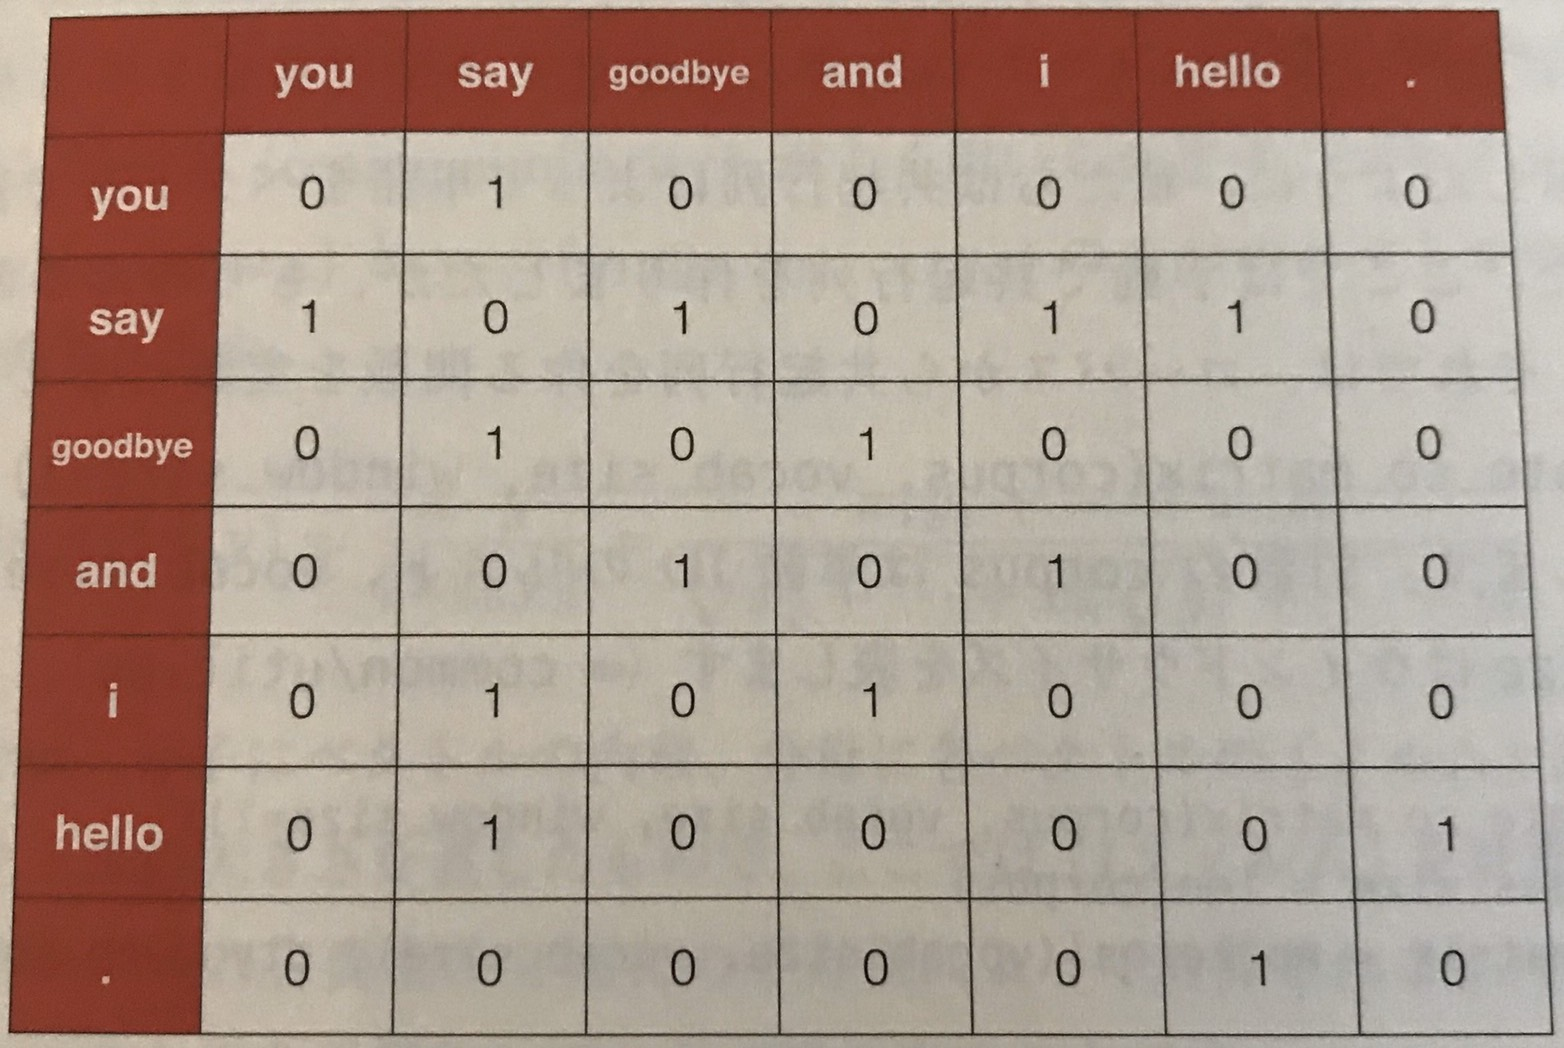
\includegraphics[width=10cm]{./matrix.jpg}
   \caption{共起行列の表}
   \label{fig:}
 \end{center}
\end{figure}

これは共起行列と呼ばれ, それぞれの行を参照することにより各単語のベクトルを得ることができる.

\subsection{ベクトル間の類似度}
様々な手法があるが, 単語のベクトル表現の類似度に関しては次式で定義されるコサイン類似度がよく用いられる.
\begin{equation}
  similarity({\bm {x}}, {\bm {y}}) = \frac{{\bm {x}}・{\bm {y}}}{\left\lVert {\bm x} \right\rVert  \left\lVert {\bm y} \right\rVert}
\end{equation}

\subsection{単語の分散表現の改良}
 以上の共起行列では単に共起する回数に着目しているので, 「drive」と「car」よりも「the」と「car」の方が強い関連性を持ってしまう. これを改善するために以下で定義する相互情報量(Pointwise Mutual Information)という指標を使う.
\begin{equation}
  PMI(x, y) = \log_{2} \frac{P(x, y)}{P(x)P(y)}
\end{equation}
ここで, ${P(x)}$は${x}$が起こる確率, ${P(y)}$は${y}$が起こる確率, ${P(x, y)}$は${x}$と${y}$が同時に起こる確率を表す. また, PMIはその値が高いほど関連性が高いことを示す. 例えば10000個の単語からなるコーパスで「the」が1000回,「car」が20回,「drive」が10回出現し,「the」と「car」が10回共起し, 「drive」と「car」が5回共起したとする. その時, PMI("the", "car") ${\approx}$  2.32, PMI("car", "drive") ${\approx}$ 7.97となり正しく評価できている. また, 実践上では負のPMIは0にする正の相互情報量を用いる.

\subsection{次元削減}
 次元削減には様々な手法があるがここでは特異値分解(Singular Value Decomposition: SVD)を行う. 任意の行列${\bm {X}}$を, ${\bm {U}}$, ${\bm {S}}$, ${\bm {V}}$の3つに分解する. つまり,
\begin{equation}
  \bm {X = USV}^T
\end{equation}
ここで${U}$と${V}$は直行行列でありその列ベクトルは互いに直交する. ${S}$は対角行列であり, 対応する軸の重要度を示す特異値が降順に並んでいるので特異値が大きいものに対応する軸のみ残すことで次元削減が可能になる.

\subsection{カウントベースの手法の問題点}
現実的にはコーパスで扱う語彙数は非常に巨大で語彙数が100万をゆうに超えると言われている. その際カウントベースの手法では100万\times 100万の巨大な行列をつくることになり, n\times nの行列に対して${O(n^3)}$の計算量がかかる特異値分解は現実的ではない.

\section{推論ベースの手法}
推論ベースの手法では, 周囲の単語(コンテキスト)が与えられたときにどのような単語が出現するかを推測し, 学習する. その学習の結果として単語の分散表現を得られるというのが推論ベースの手法である.

\subsection{word2vec}
単語はone-hotベクトル化することで入力されるニューロンを固定長のベクトルにすることが可能. これをモデルへの入力とするが, continuous bag-of-words(CBOW)と呼ばれるモデルを使う. 以下にその概要を示した.

\begin{figure}[!htbp]
 \begin{center}
   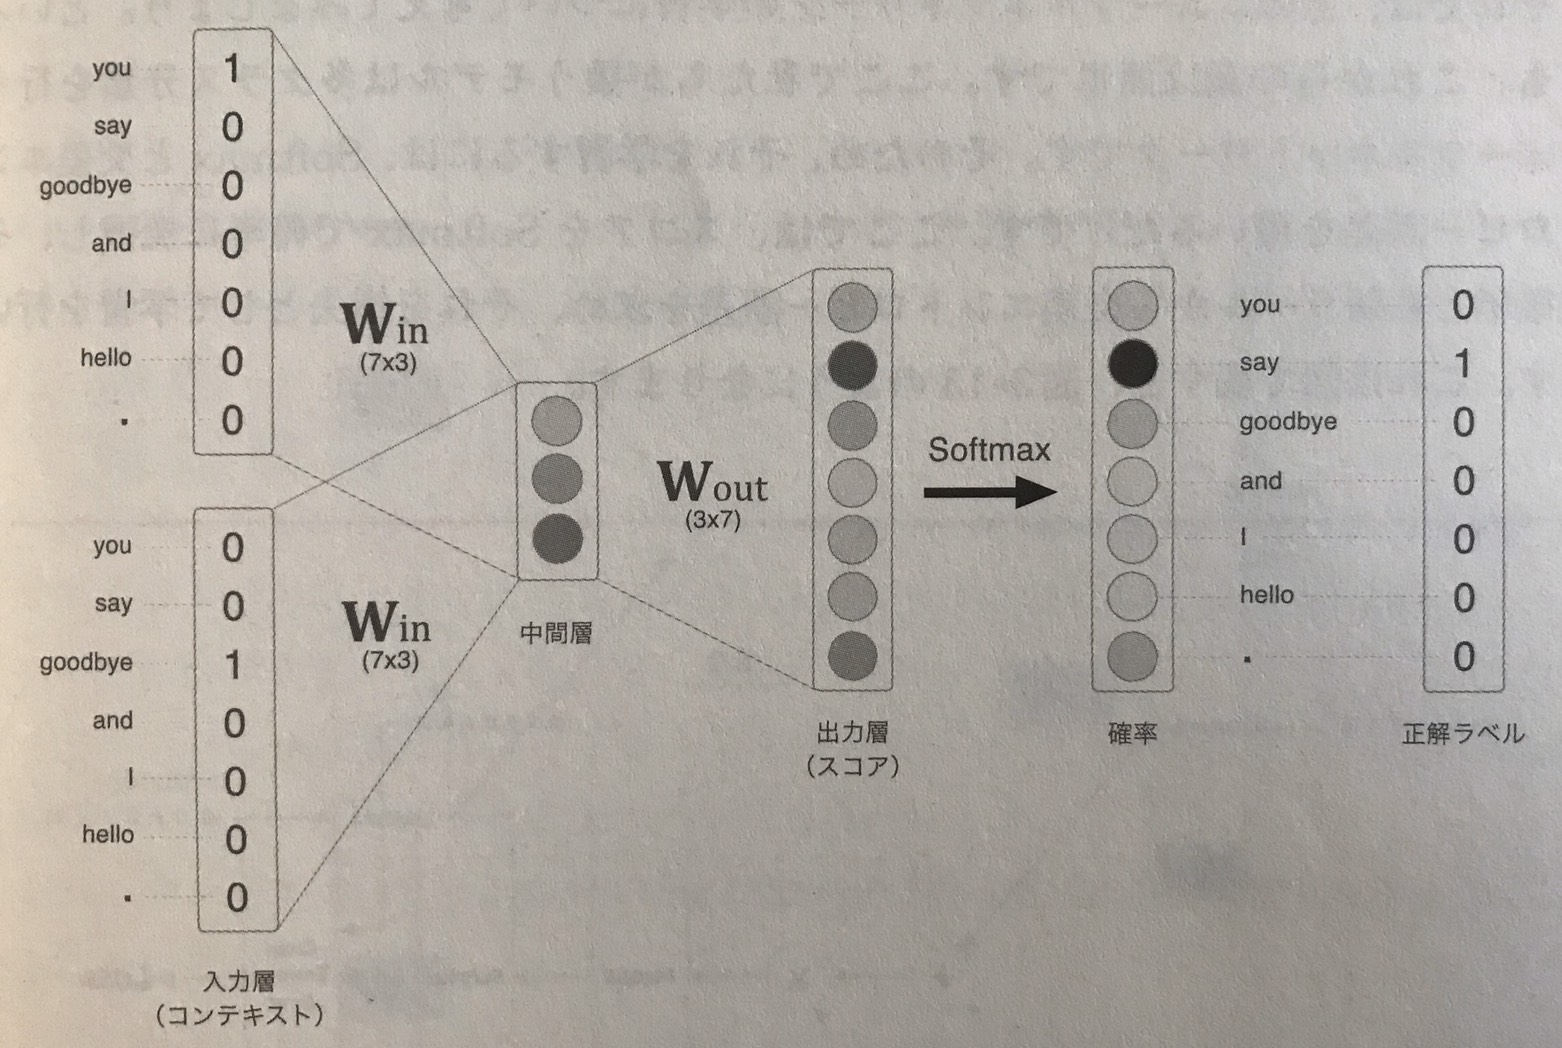
\includegraphics[width=8cm]{./CBOW.jpg}
   \caption{CBOWモデルのネットワーク構造}
   \label{fig:}
 \end{center}
\end{figure}

注意すべきは中間層にあるニューロンは各入力層の全結合による変換後の値が相加平均されていることである. 最終的な出力は各単語のスコアであり, Softmax関数を適用することで単語の出現確率が求められる. 損失関数は, 多くの場合交差エントロピー誤差を用いる.
最終的に利用する単語の分散表現は, 多くの研究では入力側の重み${W_{in}}$だけを利用する.

\subsection{CBOWモデルの逆伝播}
CBOWモデルの逆伝播を図解すると以下の通りである.
\begin{figure}[!htbp]
  \begin{center}
    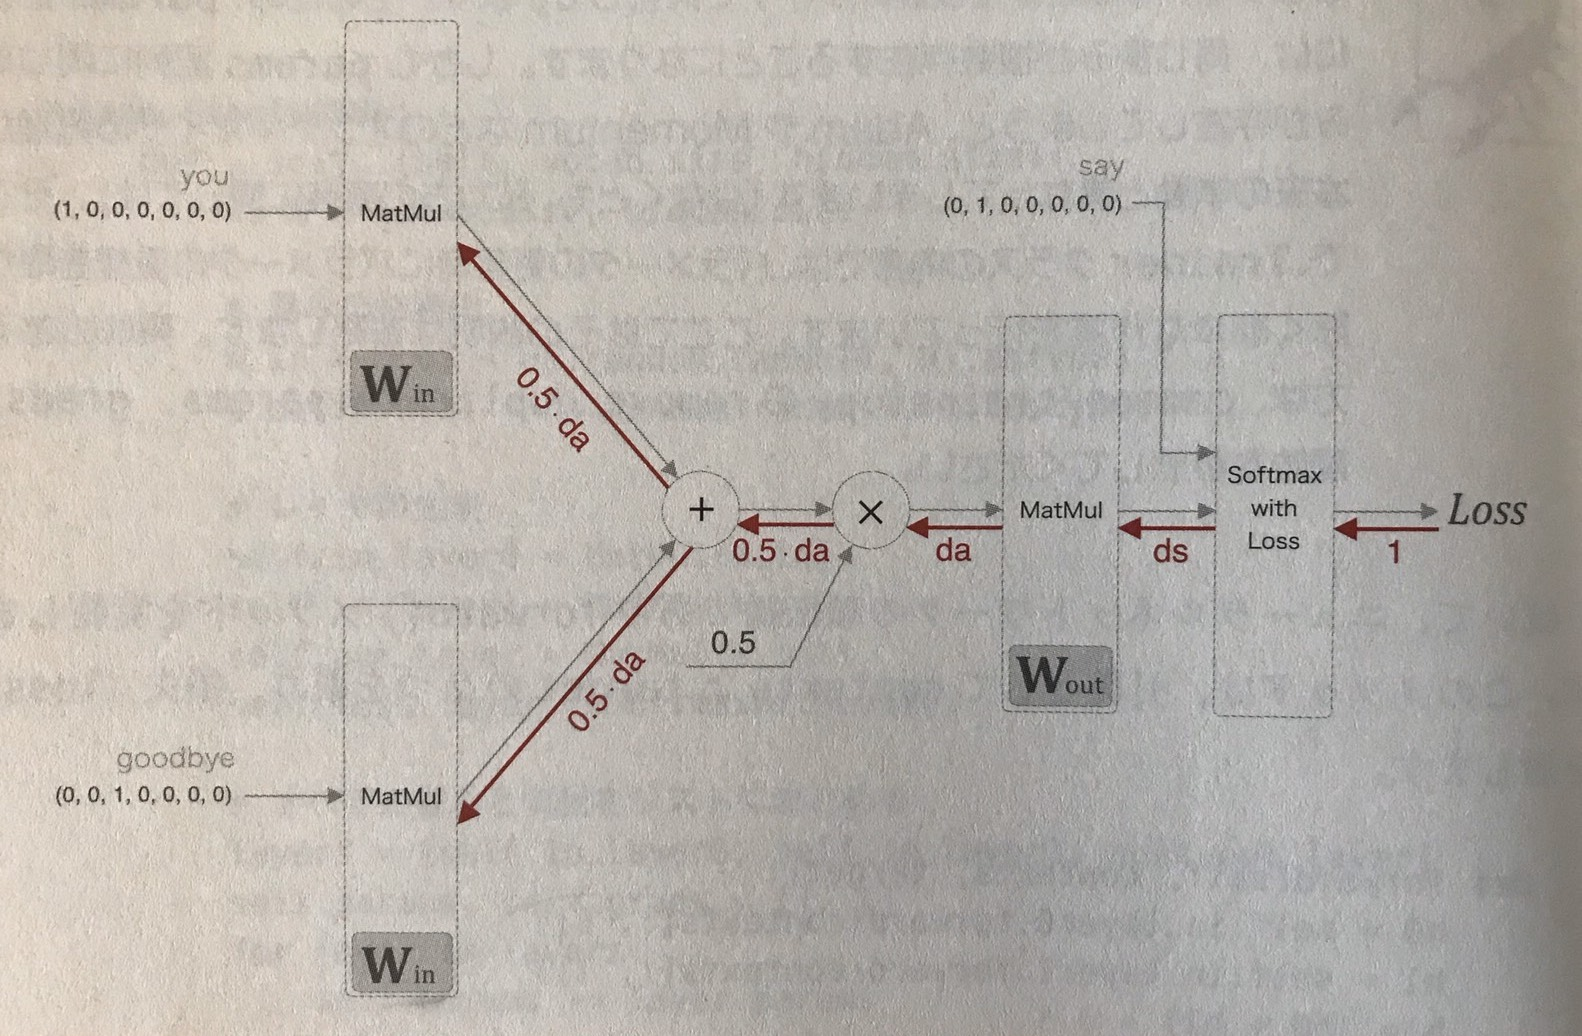
\includegraphics[width=8cm]{./CBOW_bp.jpg}
    \caption{CBOWモデルの逆伝播}
    \label{fig:}
  \end{center}
\end{figure}

Softmaxノードと交差エントロピー誤差を結合した場合, 逆伝播は出力層のインデックスをkとすると,
\begin{equation}
  ds = (y_k - t_k)
\end{equation}
となる.[2][3]
よって, 中間層のインデックスをjとすると, ${\bm {W_{out}}}$の誤差逆伝播は,
\begin{equation}
  \frac{\partial E}{\partial w^{out}_{jk}} = x_j (y_k - t_k)
\end{equation}
である. [3] また,
\begin{equation}
  \frac{\partial E}{\partial x_j} = \sum_{k} (y_k - t_k)w^{out}_{jk}
\end{equation}
である[3]. これを用いて
\begin{eqnarray}
  \frac{\partial E}{\partial W_{in}} = 0.5 \times \frac{\partial E}{\partial X} \times W^T_{in}
\end{eqnarray}
で求められる.


\subsection{CBOWモデルの確率的表現}
コーパスを${w_1, w_2, \dots, w_T}$で表現するとする. コンテキストとして${w_{t-1}}$, ${w_{t+1}}$が与えられたときに, ターゲットが${w_t}$となる確率は
\begin{equation}
  P(w_t|w_{t-1}, w_{t+1})
\end{equation}
で表される. これは「${w_{t-1}, w_{t+1}}$が与えられたときに${w_t}$が起こる確率」を表しているのでCBOWモデルを表現しているといえる. 損失関数である交差エントロピーも${L = - \sum_{k} t_k \log y_k }$であり, ${t_k}$がone-hotベクトルの教師ベクトルであることに注意すると
\begin{equation}
  L = - \log P(w_t|w_{t-1}, w_{t+1})
\end{equation}
となる. これは単に確率に対数をとって−1倍したものである. これを一つのサンプルデータからコーパス全体に拡張することで損失関数は以下のようになる.

\begin{equation}
  L = - \frac{1}{T} \sum^{T}_{t=1} \log P(w_t|w_{t-1}, w_{t+1})
\end{equation}
CBOWモデルの学習で行うことは, この損失関数をできる限り小さくすることである. そしてその時の重みパラメータが目的とする単語の分散表現である.


\subsection{skip-gramモデル}
word2vecではCBOWモデルの他にskip-gramモデルが提案されている. CBOWモデルは周囲の単語から中央の単語を予測するのに対し, skip-gramモデルでは中央の単語から周囲の単語を予測する.

\begin{figure}[!htbp]
 \begin{center}
   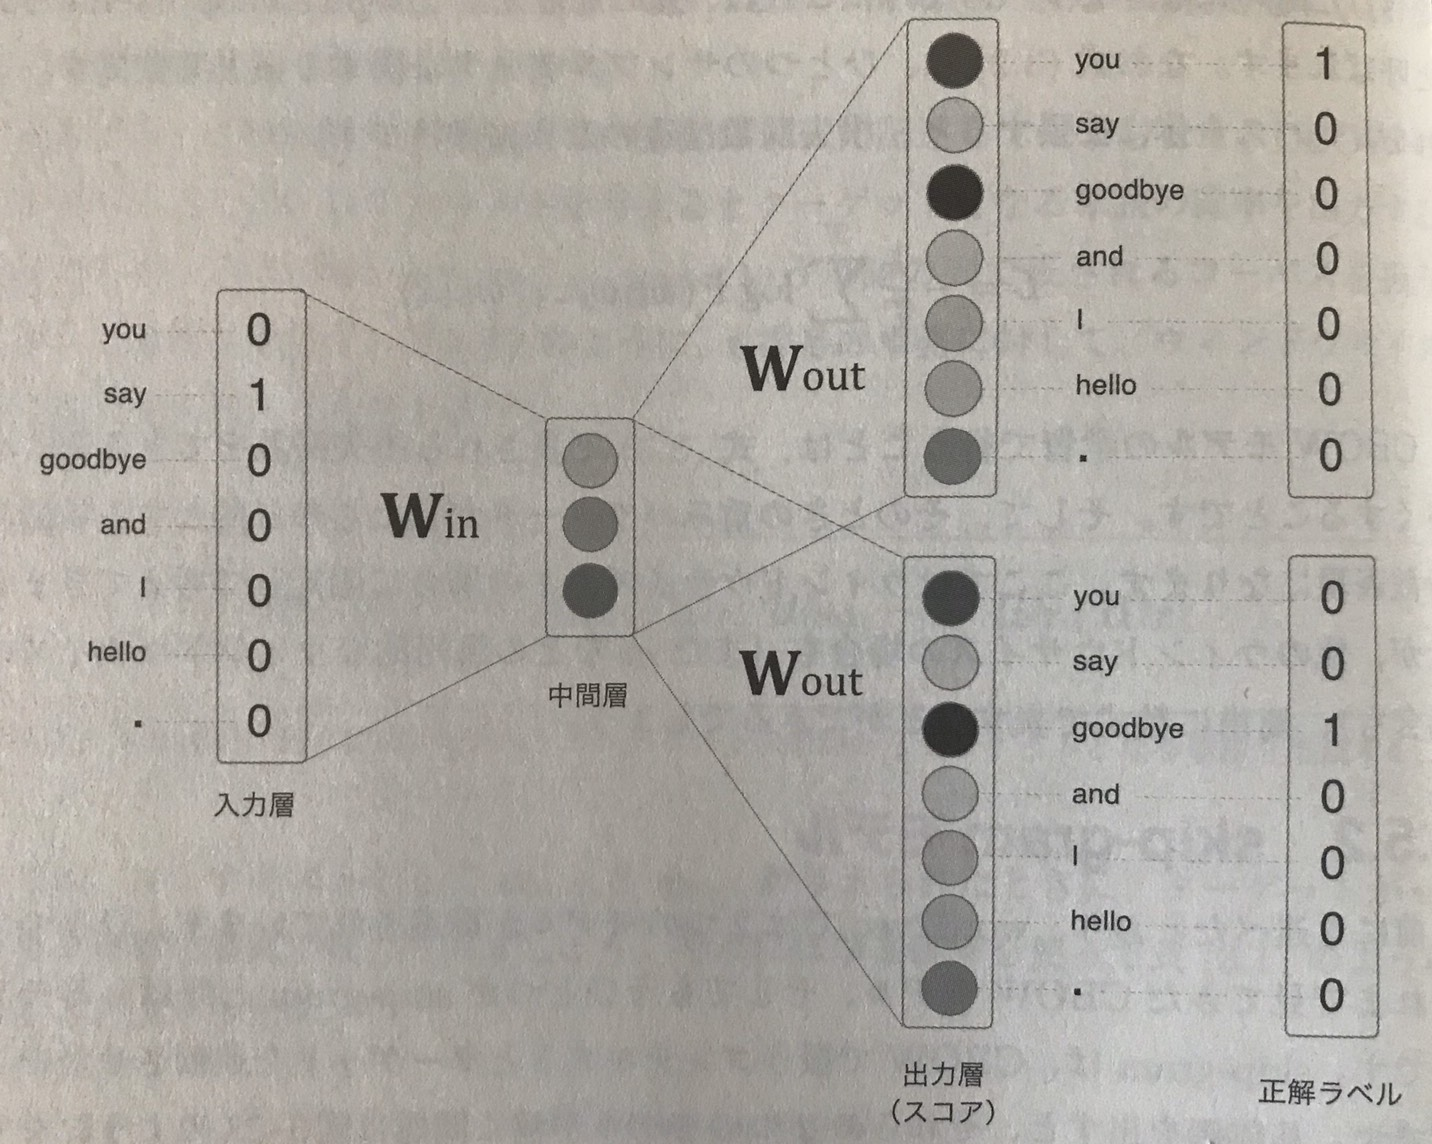
\includegraphics[width=8cm]{./skip_gram.jpg}
   \caption{skip-gramモデルのネットワーク構造}
   \label{fig:}
 \end{center}
\end{figure}

CBOWモデルと同様に確率の表記で表現する. まず, 単語の予測は次の確率で表現される.
\begin{equation}
  P(w_{t-1}, w_{t+1}|w_t) = P(w_{t-1}|w_t)P(w_{t+1}|w_t)
\end{equation}
これを交差エントロピー誤差に適用することでskip-gramモデルの損失関数が次のように導ける.
\begin{eqnarray}
  L &=& - \log P(w_{t-1}, w_{t+1}|w_t) \nonumber \\
    &=& - \log P(w_{t-1}|w_t)P(w_{t+1}|w_t) \nonumber \\
    &=& - (\log P(w_{t-1}|w_t) + \log P(w_{t+1}|w_t))
\end{eqnarray}
これをコーパス全体に拡張することにより
\begin{equation}
  L = - \frac{1}{T} \sum^{T}_{t=1} (\log P(w_{t-1}|w_t) + \log P(w_{t+1}|w_t))
\end{equation}
が導かれる.
コーパスが大規模になるにつれて低頻出の単語や類推の性能の点においてskip-gramモデルの方が優れている. 一方で, 学習速度の点ではCBOWモデルの方が優秀である.

\section{カウントベース v.s. 推論ベース}
単語の分散表現の更新作業が発生した場合, カウントベースの手法はゼロから計算を行う必要があるのに対し, 推論ベースはパラメータを再学習するときに初期値を以前のものに設定することで効率的に学習が行える.
カウントベースの手法では主に単語の類似性がエンコードされる
推論ベースの手法では単語の類似性に加えて複雑な単語間のパターンも捉えられる(word2vecは「king - man + woman = queen」が解ける.)
しかし, 推論ベースとカウントベースは優劣がつけられれないことが報告されている.


\begin{thebibliography}{9}
  \bibitem{教科書} 斎藤康穀. ゼロから作るDeep Learning 2. p57-129
  \bibitem{Qiita} 【機械学習】誤差逆伝播法による速度改善(その2). https://qiita.com/m-hayashi\\/items/fa4749f8080e542787d2
  \bibitem{Qiita} 【機械学習 誤差逆伝播法】word2vecメモ (1) https://qiita.com/sand/items/85ea76f9c26aabb849e7
  \bibitem{論文} Improving Distributional Similarity with Lossons Learned from Word Embeddings https://www.aclweb.org/anthology/Q15-1016/
\end{thebibliography}
\end{document}
